% \section{BIODATA PENULIS}

% Bagian Judul
\begin{center}
    {\LARGE\bfseries BIODATA PENULIS}
    \vspace{2em}
\end{center}

% Bagian Lingkungan Gambar Berbalut Teks
% {l} artinya gambar diletakkan di sebelah kiri (left)
% {0.38\textwidth} adalah lebar ruang untuk gambar (sekitar 38% dari lebar teks)
\begin{wrapfigure}{l}{0.30\textwidth}
    \vspace{-15pt} % Mengatur jarak vertikal ke atas agar foto sejajar dengan baris pertama teks
    \centering
    % Ganti 'foto_anda.jpg' dengan nama file foto Anda yang sebenarnya
    % Jika belum ada fotonya, Anda bisa gunakan \rule{\linewidth}{7.5cm} sebagai placeholder sementara
    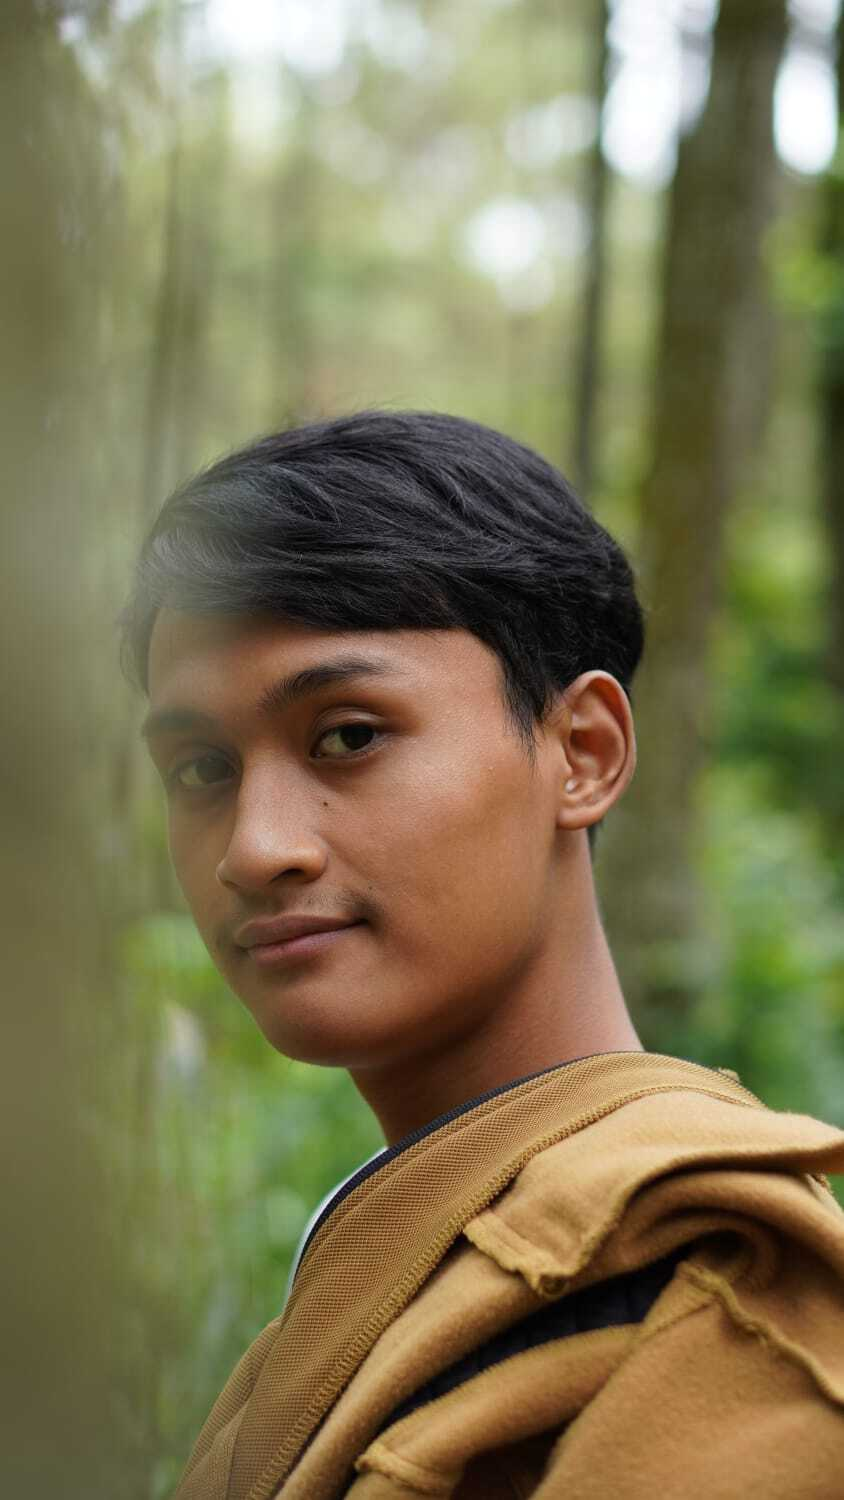
\includegraphics[width=\linewidth]{konten/foto_gweh.jpg} 
    \vspace{-10pt} % Mengatur jarak vertikal ke bawah sebelum teks di bawah foto kembali normal
\end{wrapfigure}

Penulis bernama Ilham Rasyid Machfudi, biasa dipanggil Ilham, lahir di Malang, 31 Januari 2004. Penulis merupakan anak ke 2 dari 3 bersaudara. Penulis menempuh pendidikan formal di SDN 1 Sidokumpul Gresik, SMPN 3 Gresik, SMAN 1 Manyar Gresik, dan kuliah 
tingkat sarjana di Departemen Fisika ITS. Penulis mengambil bidang minat fisika teori dan masuk menjadi mahasiswa S1 ITS tahun 2022 melalui jalur SBMPTN dengan NRP 5001221124. Selama perkuliahan, dalam bidang non-akademik, penulis aktif berkontribusi dalam pengembangan pelayanan asisten laboratorium Fisika Laboratorium II. 
Penulis berharap penelitian ini dapat bermanfaat dan dikembangkan lebih lanjut. Jika ada pertanyaan 
seputar penelitian ini, penulis dapat dihubungi melalui email ilrasyid5@gmail.com.